\clearpage
\section{Fitting a Parametric Function for Looping}
\label{sec:fit-par}


We follow \citet{hoffmann2022trainingcomputeoptimallargelanguage} setup for fitting a parametric loss function. Specifically, using the models trained with several IsoFLOP budgets in \cref{sec:train-scaling}, we fit a parametric function of the form
\begin{equation}
    \widehat{\mathcal{L}}_{\text{train}}(\mu_{\text{rec}}, \mathcal{D}) = E + A \cdot \mathbf{N}(\mu_{\text{rec}})^{-a} + B \cdot \mathcal{D}^{-b}
\end{equation}
where $\mathbf{N}(\mu_{\text{rec}})$ is the \emph{effective parameter count} of the model if you were to unroll all loops into real parameters, $\mathcal{D}$ is the number of tokens that were used in training, and $A, B, a, b$ are learned parameters. We specifically use Huber loss \citep{huber} on the log loss between the prediction of the parametric fit and the validation loss of the models, using L-BFGS \citep{lbfgs} to minimize. We choose the parametric function of this form as it exactly follows \cite{hoffmann2022trainingcomputeoptimallargelanguage}, but with parameters $\mathbf{N}$ now being a function of \meanrecurrence. Finally, we take the best result from 500 random restarts of L-BFGS, each with up to 10,000 iterations, selecting the initialization that achieves the lowest Huber loss. The results of fitting the parametric function can be visualized in \cref{fig:parameteric-fit-app}, and the learned values can be observed in \cref{tab:parametric-fit-app}.


\begin{figure}[!h]
    \centering
    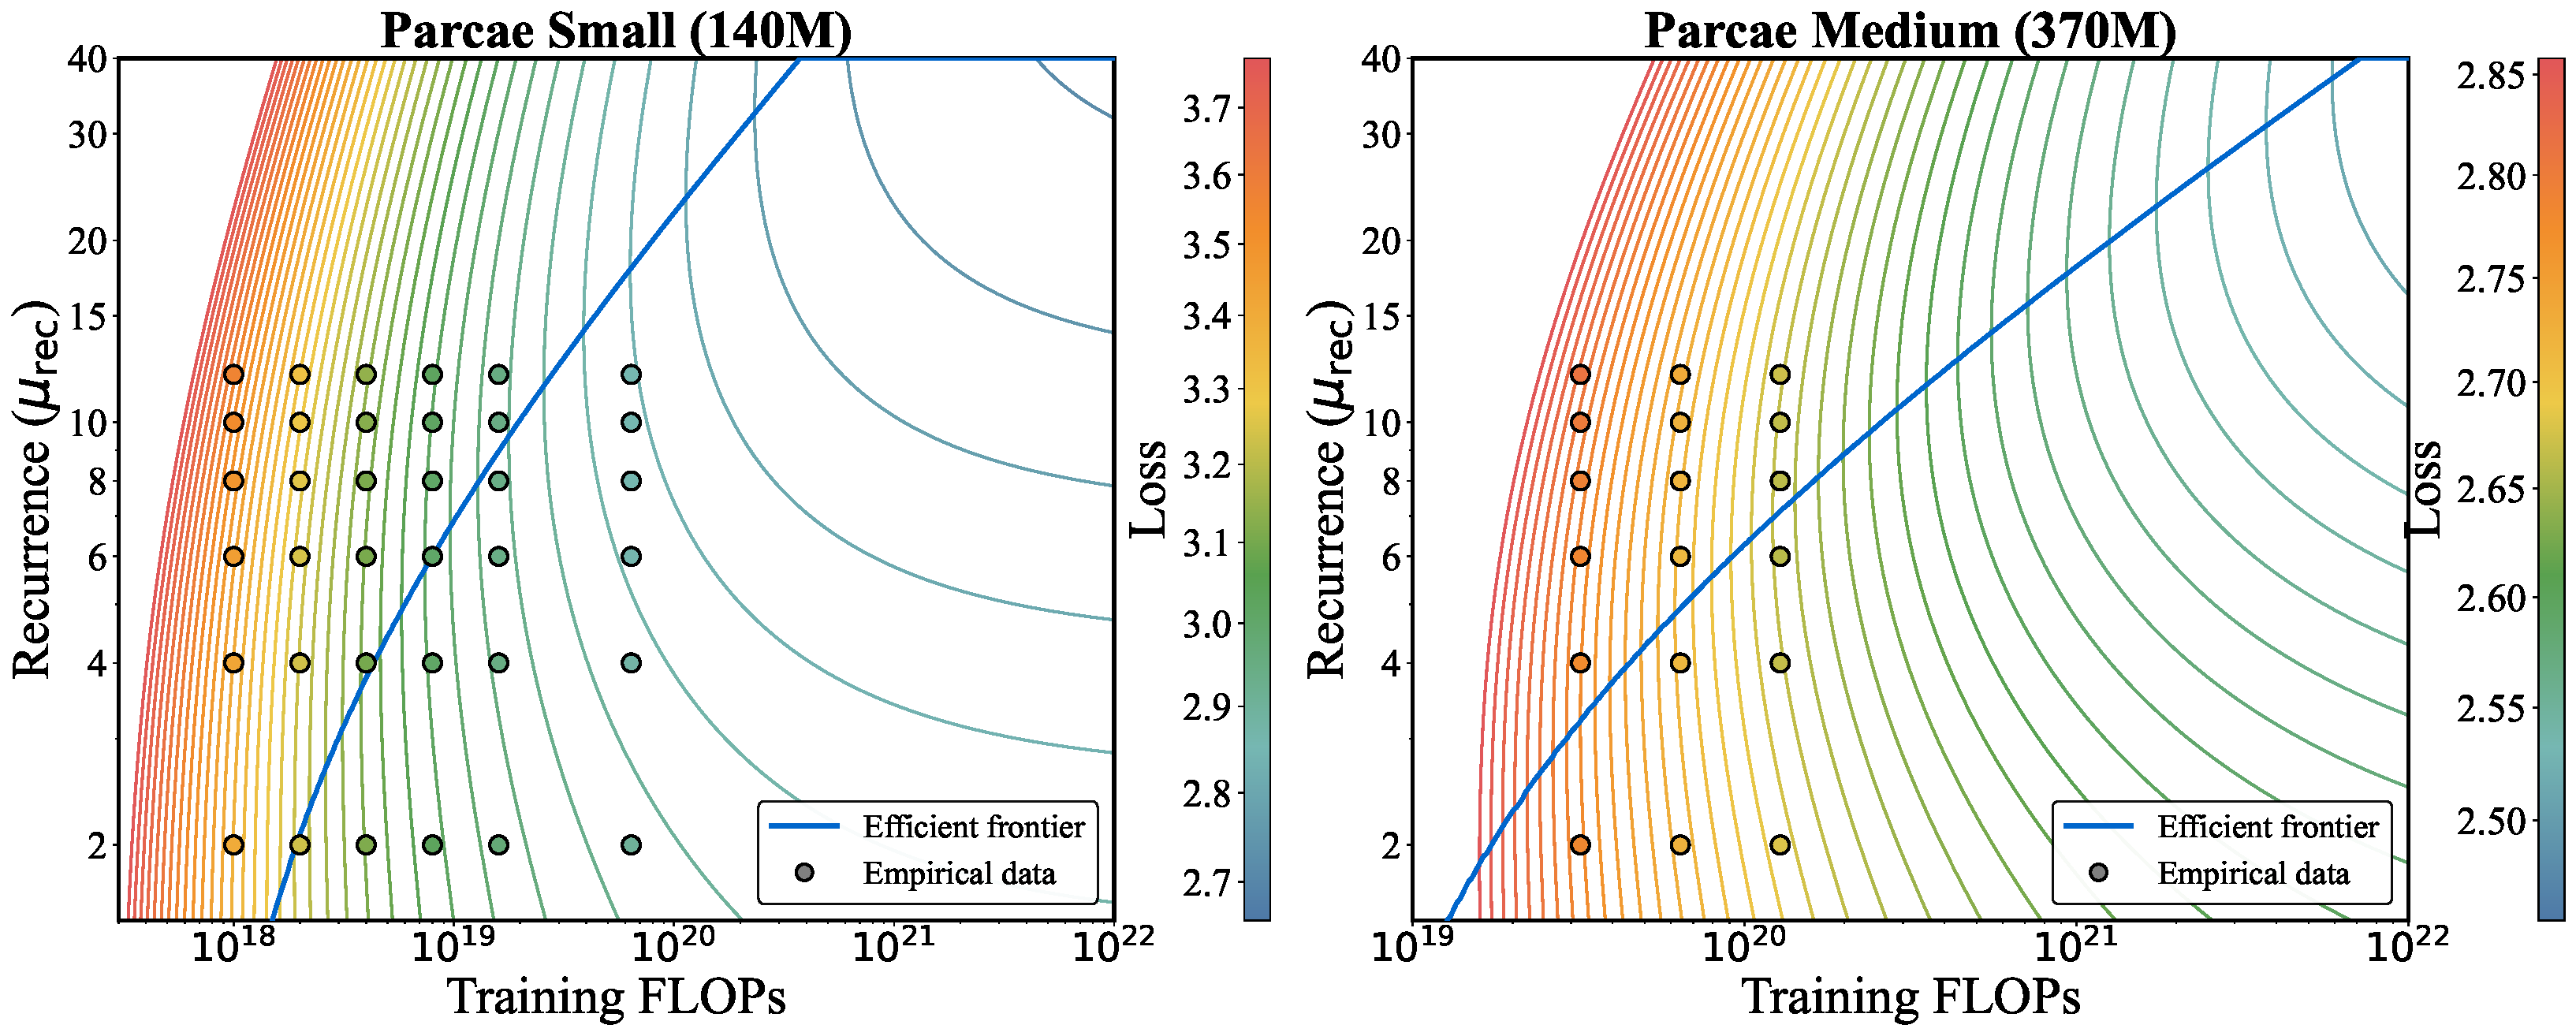
\includegraphics[width=\linewidth]{figures/appendix/parametric_fit_contours.pdf}
    \caption{\textbf{Parametric Fit of Looping.} Visualization of our parametric function $\widehat{\mathcal{L}}_{\text{train}}(\mu_{\text{rec}}, D)$, which displays the IsoLoss contours for both 140M Parcae (\emph{left}) and 370M Parcae (\emph{right}) models. }
    \label{fig:parameteric-fit-app}
\end{figure}


\begin{table}[!h]
    \centering
    \begin{tabular*}{\textwidth}{@{\extracolsep{\fill}} l|ccccccc @{}}
        \toprule
        \textbf{Model} & $\boldsymbol{E}$ & $\boldsymbol{A}$ & $\boldsymbol{a}$ & $\boldsymbol{B}$ & $\boldsymbol{b}$ & \textbf{Huber} ($\times 10^{-4}$) \\
        \midrule
        Small (140M)  & 2.662 & 522733.307 & 0.771 & 25420.102 & 0.525 & 0.44 \\
        Medium (370M) & 2.439 & 832134.346 & 0.775 & 6386.865 & 0.448 & 0.01 \\
        \bottomrule
    \end{tabular*}
    \caption{\textbf{Optimal Scaling Coefficients for Parametric Fits.}}
    \label{tab:parametric-fit-app}
\end{table}
